\documentclass[tikz,margin=2mm]{standalone}
\pagestyle{empty}

\usepackage{amsmath}
\usepackage{bm}
\usetikzlibrary{positioning,calc,arrows,arrows.meta}
\tikzset{font=\small}

\begin{document}
	% Example a True DAG
	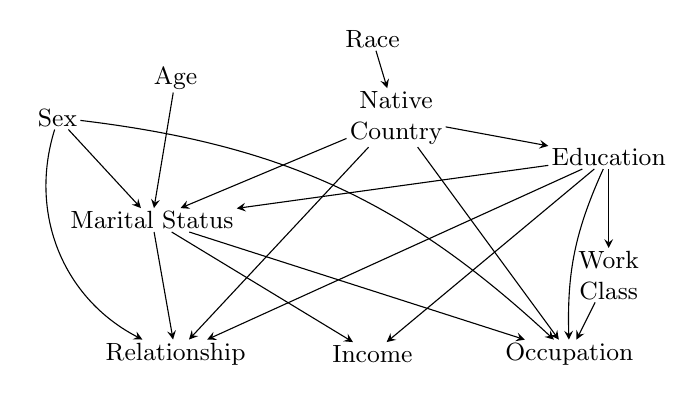
\begin{tikzpicture}
	\begin{scope}
		\tikzstyle{every node}=[align=center, inner sep=1pt]
		\node (race) at (0, 0) {Race};
		\node (native) at (0.3, -1) {Native \\ Country};

		\node (sex) at (-4, -1) {Sex};
		\node (age) at (-2.5, -0.5) {Age};
		\node (edu) at (3, -1.5) {Education};

		\node (ms) at (-2.8, -2.3) {Marital Status};
		\node (wc) at (3, -3) {Work \\ Class};

		\node (rln) at (-2.5, -4) {Relationship};
		\node (inc) at (0, -4) {Income};
		\node (occ) at (2.5, -4) {Occupation};

		\draw[->, >=stealth](race) -- (native);

		\draw[->, >=stealth](native) -- (rln);
		\draw[->, >=stealth](native) -- (ms);
		\draw[->, >=stealth](native) -- (edu);
		\draw[->, >=stealth](native) -- (occ);
		
		\draw[->, >=stealth](sex) to[bend right=40] (rln);
		\draw[->, >=stealth](sex) to[bend left=18] (occ);
		\draw[->, >=stealth](sex) -- (ms);
		\draw[->, >=stealth](age) -- (ms);
		\draw[->, >=stealth](edu) -- (ms);
		\draw[->, >=stealth](edu) -- (rln);
		\draw[->, >=stealth](edu) -- (inc);
		\draw[->, >=stealth](edu) to[bend right=13] (occ);
		\draw[->, >=stealth](edu) -- (wc);

		\draw[->, >=stealth](ms) -- (rln);
		\draw[->, >=stealth](ms) -- (inc);
		\draw[->, >=stealth](ms) -- (occ);
		\draw[->, >=stealth](wc) -- (occ);
	\end{scope}
	\end{tikzpicture}
\end{document}
